\hypertarget{correlation-based-models}{%
\section{Correlation-Based Models}\label{correlation-based-models}}

Given a global map, one type of sensor model is to correlate a local
sensor based map with a global map. \emph{Map Matching}. It is tied with
map building and localization. This is described later in detail.
Preliminaries

\begin{itemize}
\tightlist
\item
  Assume that you have a occupancy grid map \(m\).
\item
  Assume that this is a simple map with grid cells marked as occupied or
  not - binary map.
\item
  Store the map in an array \(m[i][j]\).
\item
  Let \(x_t = (x,y,\theta)\) be the robot's pose.
\item
  Let \(z_t^k\) be the range value of a sensor reading.
\item
  Let \(x_{k,\mbox{sens}}, y_{k,\mbox{sens}}\) be the location of the
  sensor in the local coordinates.
\item
  Let \(\theta_{k,\mbox{sens}}\) be the angle of the beam from the local
  (robot) coordinate system.
\item
  Use sensors to build a local map \(m_{\mbox{local}}[i_L][j_L]\)
\item
  Correlate local and global coordinate systems:
  \(\begin{pmatrix}x & y & \theta\end{pmatrix}^T\)
\end{itemize}

\begin{figure}
\centering
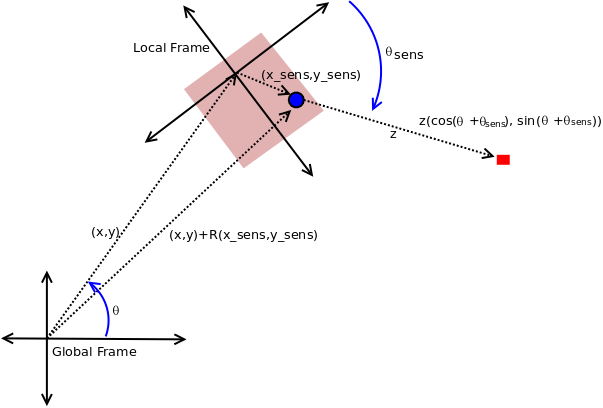
\includegraphics[width=0.5\textwidth,height=\textheight]{LocalizationFigures/coords.png}
\caption{Coordinate transforms to relate observed obstacle to global
map.}
\end{figure}

\[\begin{aligned}
\begin{pmatrix} x_{z_t^k}\\y_{z_t^k} \end{pmatrix} =
  \begin{pmatrix}x \\ y \end{pmatrix} + \begin{pmatrix} \cos\theta &
    -\sin\theta \\ \sin\theta & \cos\theta\end{pmatrix}
     \begin{pmatrix}x_{k,\mbox{sens}}\\y_{k,\mbox{sens}}\end{pmatrix}
     + z_t^k \begin{pmatrix}\cos (\theta + \theta_{k,\mbox{sens}}) \\
     \sin (\theta + \theta_{k,\mbox{sens}})\end{pmatrix}
\end{aligned}\]

\begin{itemize}
\tightlist
\item
  Find the correlation between the two spatially aligned maps on the
  common regions of definition.

  \begin{itemize}
  \item
    List out the map as a vector \(v[k] = m[i][j]\) where \(k=n*j+i\).
  \item
    Plot them as vectors and compare, how close?
  \item
    Using the average of the two, show you can get a better comparison
    by subtracting off the average.
  \item
    Find the angle between the two differenced vectors.
  \item
    Thus
    \(\overline{m} = \frac{1}{2N} \sum \left( m[i][j] + m_{\mbox{local}}[i][j]\right)\).
  \item
    Define

    \[\rho = \frac{(m - \overline{m})\cdot (m_{\mbox{local}} -\overline{m})}{\|m - \overline{m}\| \| m_{\mbox{local}} -\overline{m}\|}\]
  \item
    Define \(p(m_{\mbox{local}}|x_t,m) = \max \{\rho , 0\}\)
  \end{itemize}
\end{itemize}

Can you do template matching on this? How about ICP?

\begin{figure}
\centering
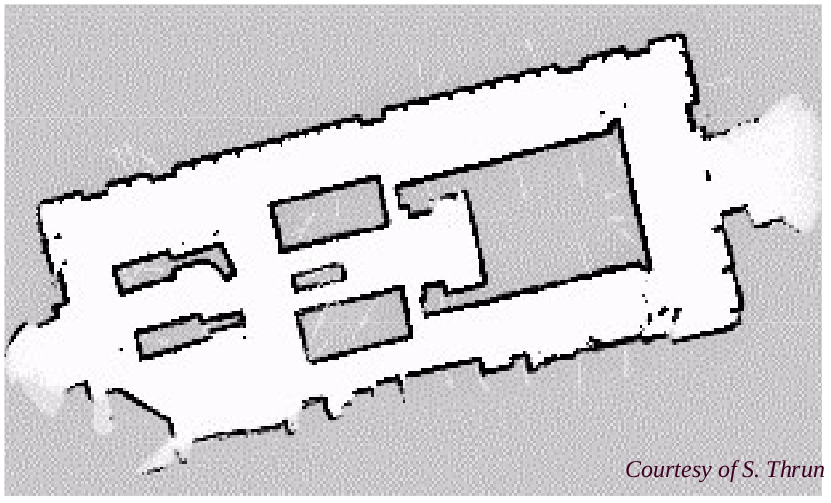
\includegraphics{LocalizationFigures/map5.png}
\caption{}
\end{figure}

Where does this fit:

\begin{figure}
\centering

\includegraphics{LocalizationFigures/map5_cut.png}
\caption{}
\end{figure}

\textbf{Extract features from measurements.}

This is similar to what is done in computer vision.

\begin{itemize}
\tightlist
\item
  Identify features which correspond to distinct objects, call them
  landmarks.
\item
  Assume you can obtain a range and bearing for the landmark.
\item
  Call the unique identifier for a landmark, a signature.
\item
  For the \(i^{th}\) measurement at time \(t\), denote range by
  \(r^i_t\), bearing \(\phi^i_t\) and signature \(s^i_t\).
\end{itemize}

\emph{Feature based map}: \(m = \{ m_1, m_2, \dots \}\). The \(j^{th}\)
map feature be defined by \(m_j = (m_{j,x}, m_{j,y}, s_j)^T\). The
\(i^{th}\)

feature then can be correlated to the \(j^{th}\) landmark.

Let the robot pose given by \(x_t = (x, y, \theta)^T\). Then we have:

\[\begin{aligned}
\begin{array}{l} r^i_t = \sqrt{(m_{j,x}-x)^2+(m_{j,y}-y)^2} +
\epsilon_{\sigma_r^2}\\[8pt] \displaystyle \phi^i_t =
\tan^{-1}\frac{m_{j,y}-y}{m_{j,x}-x}-\theta +
\epsilon_{\sigma_{\phi}^2}\\[8pt] s^i_t = s_j + \epsilon_{\sigma_s^2}
\end{array}
\end{aligned}\]

\emph{Data association problem} A key problem is the association of
features to landmarks.

\begin{itemize}
\item
  Introduce a \emph{correspondence variable} between feature \(f_t^i\)
  and landmark \(m_j\): \(c^i_t \in \{ 1, 2, 3,
  \dots , N+1\}\) where \(N\) is the number of landmarks in the map.
\item
  If \(c^i_t = j \leq N\) then the \(i^{th}\) feature observed at time
  \(t\)

  corresponds to the \(j^{th}\) landmark in the map. {[}\(c^i_t\) is the
  true identity.{]}
\item
  If \(c^i_t = N+1\) then the feature does not correspond to a landmark
  in the map.
\end{itemize}

To compute the probability of a feature corresponding to known landmark:

\begin{enumerate}
\tightlist
\item
  \(j=c^i_t\)
\item
  \(\hat{r}^i_t = \sqrt{(m_{j,x}-x)^2+(m_{j,y}-y)^2}\)
\item
  \(\hat{\phi}^i_t =\displaystyle\mbox{atan}\left(\frac{m_{j,y}-y}{m_{j,x}-x}\right) - \theta\)
\item
  \(q = \mbox{Gauss}(r^i_t-\hat{r})\mbox{Gauss}(\phi^i_t-\hat{\phi}) \mbox{Gauss}(s^i_t-\hat{s})\)
\end{enumerate}
